\chapter{Aspects of spine orthopedics}

In this work, I develop a model for automatic segmentation of \acrfull{ct} and \acrfull{mri} images of the lumbar spine.
In this chapter, I introduce these terms\footnote{This work is not a medical desideration. For in-depth knowledge on the anatomy and physiology of the spine, contact a specialist.}.
Secondly, I give a basic overview of the medical imaging techniques. 
Finally, there is a section on a specific medical procedure in which this information is used: the minimally invasive surgery of a spinal hernia.
The inspiration for this Master Thesis subject comes from the REISS project.
The REISS project is a joint effort of \textsc{Verhaert NP\&S}\footnote{Verhaert NP\&S is my employer.} and \textsc{imec} to support this specific procedure. 

\section{Anatomy of the human spine}

\todo[inline]{Assure all citations are ok.}


The spinal column, vertebral column or backbone \footnote{NL: \textit{wervelkolom}} is a structure of 34 bones. 
It holds the body upright while providing it with the mobility to bend and twist.
Moreover, the vertebral column serves as a conduit for major nerves running from the brain to the tips of the toes.
The spinal colum, as illustrated in figure \ref{fig:spineimage} can be divided into 5 regions:
\begin{description}
    \item[the Cervical spine:] 7 vertebrae of the neck, indicated by C$_1$ to C$_7$\footnote{The vertebrae are always numbered from the head down. C1 (\textit{atlas}) is the vertebra closest to the head}.
    \item[the Thoracic spine:] 12 vertebrae of the middle back (T$_1$ to T$_{12}$).
    \item[the Lumbar spine:] 5 vertebrae that form the lower back. These are commonly referenced as L$_1$ to L$_5$.
    \item[the Sacrum:]\footnote{NL: \textit{Heiligbeen}} This is a structure consisting of 5 naturally fused vertebrae (S$_1$-S$_5$).
    \item[the Coccyx:]\footnote{NL: \textit{Stuit of staartbeen}} Structur of 4 naturally fused vertebrae at the end of the spinal column.
\end{description}

\marginpar{
        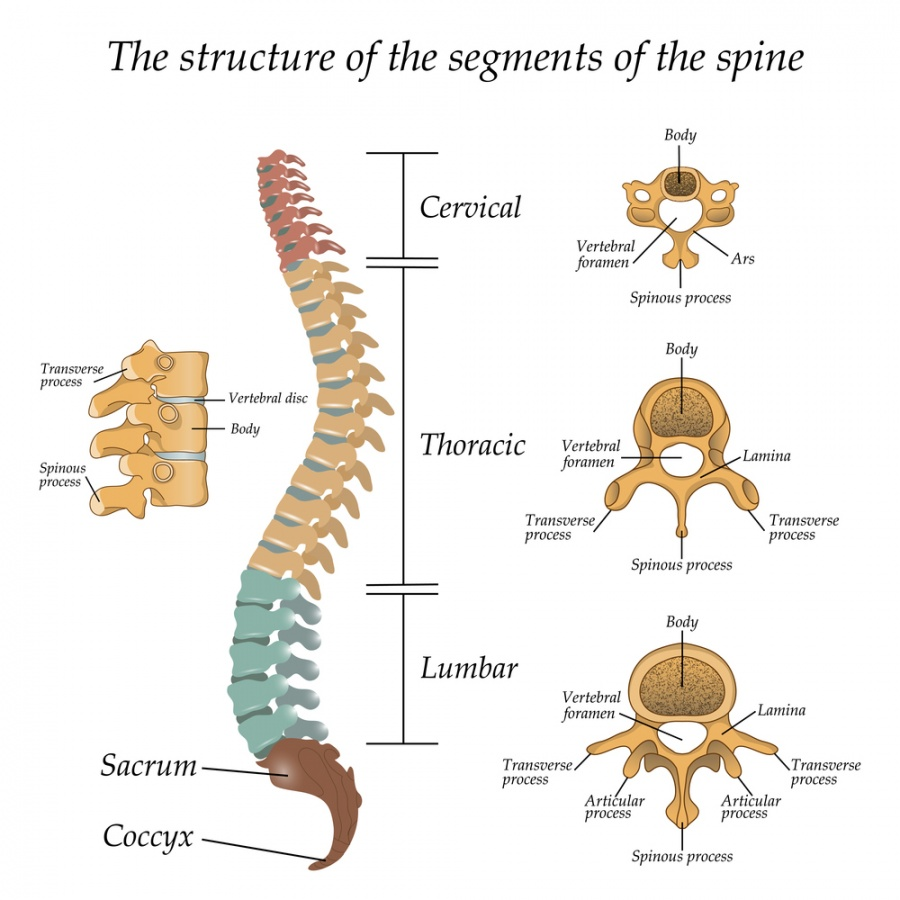
\includegraphics[width=5cm]{/home/thesis/images/SpineModel.jpeg}
        \captionof{figure}{Model of the human spine}
        \label{fig:spineimage}
    }

\todo[inline]{
    Add explanation of the causes of spinal hernia: tussenwervelschijven, zenuwknelling. 
    Ook een afbeelding van scoliose toevoegen, want sommige datasets bevatten patienten met scoliose.}

\clearpage

\section{Medical imaging of the human spine}

\todo[inline]{Describe Hounsfield scale.}

For spinal pathology diagnosis of the \hlnote{main}{Is this correct? Find reference.} medical imaging techniques are \acrfull{ct}, \acrfull{us} and \acrfull{mri}. 
These techniques allow non-invasive visualization of the spine and discs in three dimensions.

Slices from these volumetric scans are illustrated in \ref{fig:mri_ct}.

\marginpar{
        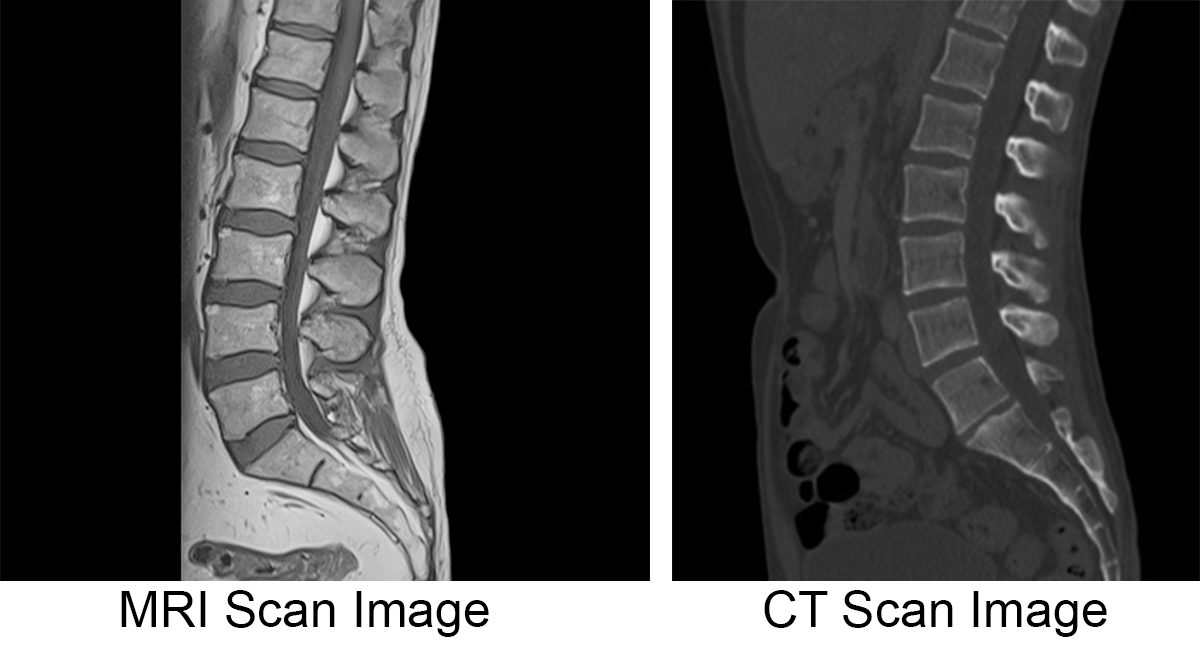
\includegraphics[width=5cm]{/home/thesis/images/MRI_CT_images.jpeg}
        \captionof{figure}{Illustration of \acrshort{ct} and \acrshort{mri} images of a human lumbar spine.}
        \label{fig:mri_ct}
    }

\section{Minimally invasive surgery of spinal hernia}